\documentclass[prd,preprintnumbers,floatfix,
nofootinbib,superscriptaddress]{revtex4}

%------------------

\usepackage{float}
\usepackage{nicefrac}
\usepackage{mathtools}
\usepackage{amsfonts}
\usepackage{amssymb}
\usepackage{amsmath}
\usepackage{graphicx}
\usepackage{subfigure}
\usepackage{array}
\usepackage{dcolumn}
\usepackage{bm}
\usepackage{esint}
\usepackage{xcolor}
\usepackage{longtable} % long tables
\usepackage{hyperref}
\usepackage{verbatim}
\usepackage{epsfig}
\usepackage{slashed}
\usepackage{color}
\usepackage{todonotes}


\newcommand{\diff}{\mathrm{d}}
\newcommand{\ket}[1]{\ensuremath{\left|#1\right\rangle}}
\newcommand{\bra}[1]{\ensuremath{\left\langle #1\right|}}
\newcommand{\braket}[2]{\ensuremath{\left\langle #1|#2\right\rangle}}
\newcommand{\TS}{\mathrm{TS}}
\newcommand{\LLH}{\mathrm{LLH}}
\newcommand{\M}{\mathcal{M}}
%
\newcommand{\I}{\ensuremath{I}}
\newcommand{\II}{\ensuremath{{I\!I}}}
\newcommand{\III}{\ensuremath{{I\!I\!I}}}
\newcommand{\IV}{\ensuremath{{I\!V}}}

\graphicspath{{../plots/}{figs/}}

\begin{document}
\title{Parity and signature test for the vector-vector system (revisited)}

%%%%%%%%%%
\author{Mikhail Mikhasenko}
\email[e-mail: ]{mikhail.mikhasenko@cern.ch}
\affiliation{CERN-EP, CH-1211, Geneva, Switzerland}
%%%%%%%%%%

%%%%%%%%%%
\date{\today}
%%%%%%%%%%

%%%%%%%%%%
\begin{abstract}
  We present a construction of the reaction amplitude
  for inclusive production of a resonance decaying to a pair of identical vector particles such as $J/\psi J/\psi$, $\phi\phi$, $Z^0 Z^0$.
  The method provides possibility of determining the spin and parity of a resonance in a model-independent way.
  A test of the methodology is demonstrated using the Standard Model decay of the Higgs boson to four leptons.
\end{abstract}
%%%%%%%%%%

\nopagebreak
\maketitle

\definecolor{cola}{rgb}{0.9,0.62,0.0}
\definecolor{colb}{rgb}{0.337, 0.706, 0.914 }
\definecolor{colc}{rgb}{0.0, 0.62, 0.451}
%
\newcommand{\mishatodo}[1]{\todo[inline,backgroundcolor=colb!50!white]{\textbf{Misha:} #1}}
\newcommand{\misha}[1]{{\color{colb} \textit{Misha:} #1}\xspace}
%

\section{Introduction}

Formation of the hadronic matter is the one of a few poorly understood parts of Quantum Chromodynamics (QCD) leaving a little black spot in the Standard Model.
While the QCD is the fundamental theory of strong interaction,
it operates with the other degrees of freedom that those at low energy where hadronic phenomena emerge.
The constituent quark model successfully describes the majority of observed hadronic states, however, far not all.
Over the last decade we have witnessed overwhelming evidence of unexpected phenomena beyond the constituent quark model that
include the observation of $XYZ$ states in the charmonium spectrum~\cite{Godfrey:2008nc}, pentaquark states~\cite{Aaij:2015tga,Aaij:2019vzc},
as well as resonance-like phenomena from the triangle singularity in hadron scattering~\cite{Alexeev:2020lvq}.
The spin-parity of the observed exotica is a critical part of the formation puzzle, and moreover, in most of the cases it can be determined experimentally.
Nevertheless, the separation of the different hypothesis is often rather cumbersome and requires case-by-case treatment.
In the paper we revisit the problem of the spin-parity assignment for the system of two identical vectors with their possible further decay.

We anticipate three applications of the presented framework.
First, to facilitate future studies of the resonance-like structures in the $J/\psi J/\psi$ spectrum
just released by LHCb~\cite{Aaij:2020xyz}.
The knowledge of quantum numbers will helping to understand the mechanism for binding of four charm quarks~\cite{Liu:2019zoy}.
% Once confirmed, the discovery sets the new milestone in the understanding of the hadron formation through the mechanism for binding four charm quarks~\cite{Liu:2019zoy}.
Second, to investigate central exclusive production (CEP) of the vector-meson pairs.
The data of the WA102 experiment on the production of $\phi\phi$ pairs
hint at a resonance signal, that is a candidate for a tensor glueball~\cite{Barberis:2000em,Lebiedowicz:2019jru}.
The proposed approach sets the ground for the complete partial wave analysis of the high statistics CEP production of four scalar mesons that should be possible with modern LHC data.
Thirdly, one find the same vector-vector signature in the Standard Model (SM) decay of the Higgs boson, $H\to Z^0Z^0$.
To conclude in favor of the $0^+$ hypothesis in Ref.~\cite{Aad:2013xqa,CMS:2018mmw}
% for the spin-parity of the Higgs boson
several phenomenological models were compared using the combined dataset of several decay channels.
In contrast, here we discuss the anatomy of the assumption-free approach.

The two key constraints that determine the properties of the decay are parity conservation and permutation symmetry.
One consequence of these constraints is known as the Landau-Yang theorem~\cite{Yang:1950rg,Landau:1948kw}.
The theorem states that a massive boson with $J^P = 1^\pm$ cannot decay into two on-shell photons.
The statement follows naturally from the general equations we provide. Moreover, the extension of the selection rule to all natural quantum numbers with odd spin is easily obtained.
A parity-signature test of a signal in the $\phi\phi$ system have been discussed in the past by several authors~\cite{Chang:1978jb,Collins:1977iv,Trueman:1978kh,Trueman:1978kh}.
We derive results consistent with the previous works using modern conventions on the state vectors and rotation matrices.
Also, we suggest exploring the spin-parity hypothesis using the full power of the multidimensional test statistics.

The paper is organized as follows. The reaction amplitude is presented in Sec.~\ref{sec:reaction.amplitude}.
In Sec.~\ref{sec:symmetries} we discuss the symmetry constraints.
We describe the test-statistics discriminator in Sec.~\ref{sec:test.statistics},
and we demonstrate the method on the SM Higgs decay in Sec.~\ref{sec:higgs}.

%                                      _|  _|    _|                      _|
%    _|_|_|  _|_|_|  _|_|    _|_|_|    _|      _|_|_|_|  _|    _|    _|_|_|    _|_|
%  _|    _|  _|    _|    _|  _|    _|  _|  _|    _|      _|    _|  _|    _|  _|_|_|_|
%  _|    _|  _|    _|    _|  _|    _|  _|  _|    _|      _|    _|  _|    _|  _|
%    _|_|_|  _|    _|    _|  _|_|_|    _|  _|      _|_|    _|_|_|    _|_|_|    _|_|_|
%                            _|
%                            _|

\section{Angular amplitude} \label{sec:reaction.amplitude}
We focus on an inclusive production process $p p'\to X + \dots$, where $X$ is a resonance decaying to two vector mesons.
Despite the vectors being identical, it is convenient to distinguish them in the reaction amplitude calling them $V_1$ and $V_2$.
In that way, we can make sure that the amplitude is symmetric on the permutation of indices $1$ and $2$.

The production frame is set up in the rest frame of $X$ as a plane that contains three-vectors of the
production reaction, i.e. $\vec p$, and $\vec p'$. The normal to the plane gives the $y$ axis (precisely $\vec p\,'\times \vec p$) as shown in Fig.~\ref{fig:production}.
We use the Gottfried-Jackson (GJ) frame for defining the $x$ and $z$ axis in the production plane~\cite{Gottfried:1964nx}.
We note that the choice of $x$ and $z$ axes is not unique: two other two common definition of the production frame are the helicity (HX) frame
defined by the direction of motion of $X$ itself in the lab frame, and the Collins-Soper (CS) frame where $z$ is defined by the bisector of the angle between $\vec p$ and $\vec p\,'$~\cite{Faccioli:2010kd}.
\begin{figure}
  \includegraphics[width=0.6\textwidth]{production_GJ.pdf}
  \caption{Schematic view of production kinematics of $X$ state at the $pp$ collider.
  The Gottfried-Jackson frame is used for describing production kinematics.
  It is defined in the rest frame of $X$ by the vectors of the beam particles:
  $\vec z = \vec p / |\vec p|$, $\vec y = \vec p' \times \vec p / |\vec p' \times \vec p|$, $\vec x = \vec y \times \vec z$.
  The spherical angles $(\theta,\phi)$ are the angles of one of two decay vectors in the GJ frame.
  The black arrows shows three dimensional vectors of particles.
  The three-momenta of the produced vectors are $\vec p_{V_1}$ and $\vec p_{V_2}$.
  }
  \label{fig:production}
\end{figure}

We consider the general case of arbitrary polarization of $X$.
We note that a negligibly small polarization is measured in the prompt production of charmonium ("head on" collisions)~\cite{Aaij:2013nlm,Chatrchyan:2012woa,CDF:2011ag, Aaij:2013oxa,Sirunyan:2018bfd}.
In opposite, for peripheral processes, e.g. central exclusive production, a significant polarization is expected~\cite{Pasechnik:2010pq}.
% For numerical tests however we restrict ourselves to the unpolarized case.

The full kinematics of the decay is described by 6 angles: a pair of spherical angles $(\theta,\phi)$ of the momentum of $V_1$ in the GJ frame, and two pairs of spherical angles $(\theta_i,\phi_i)$, $i=1,2$ for the decays of the vector mesons in their own helicity frames.
We note that the angles $\phi_i$ can also be defined in the $X$ rest frame as shown in Fig.~\ref{fig:decay} since they are not affected by the boosts along the vector-meson directions of momentum.

The spin of the decay particle $X$ defines rotational properties of the system of the decay products~\cite{Mikhasenko:2019rjf}.
Every configuration of the three-momenta of the final-state particles in the $X$ rest frame
can be considered as a solid body for which the orientation is described by three angles:
the pair of spherical angles $(\theta,\phi)$ that describe the direction of $\vec p_{V_1}$,
and $\phi_1$, the azimuthal direction of $\mu^+$ (see Fig.~\ref{fig:production} and Fig.~\ref{fig:decay}).
For definiteness, we consider the decay $X\to V(\mu^+\mu^-)V(\mu^+\mu^-)$
in the main text. A mild modifications that one needs to implement for vector decays to scalars $X\to V(S^+S^-)V(S^+S^-)$ are given in Appendix~\ref{sec:KKKK}.
The normalized differential cross section denoted by the intensity $I$ reads:
% The intensity of the decay is defined as a differential cross section over angular variables,
% $I = \diff \sigma / \diff \Omega\,\diff \Omega_1\,\diff \Omega_2$, where
% $\diff\Omega = \diff\cos\theta \diff \phi$; the $\Omega_i$, $i=1,2$ are the spherical angles of the decay products of the two vector particles in the corresponding helicity frames as shown in Fig.~\ref{fig:X.decay}.
%
% The intensity reads:
\begin{align}
    I(\Omega,\Omega_1,\Omega_2) &= (2J+1) \sum_{M,M'}R_{M,M'}\,
    \sum_{\nu,\nu'}D_{M,\nu}^{J}(\phi,\theta,\phi_1) D_{M',\nu'}^{J*}(\phi,\theta,\phi_1)
    \sum_{\xi_1,\xi_2}^{\{-1,1\}}
    A^{\nu}_{\xi_1,\xi_2}(\theta_1,\theta_2,\Delta\phi) A^{\nu'*}_{\xi_1,\xi_2}(\theta_1,\theta_2,\Delta\phi),
\end{align}
where we have explicitly separated the production and decay parts of the amplitude.
The production dynamics are encapsulated in the polarization matrix $R_{M,M'}$.
The decay amplitude is denoted by $A^{\nu}_{\xi_1,\xi_2}$
with $\nu$ being the difference of the vector-meson's helicities, and $\xi$ being the difference of the muon's helicities. $J$ and $M$ are the spin of $X$ and it's spin projection onto the $z$ axis.
The decay amplitude is described by the remaining three angles: $\theta_1$, $\theta_2$, and $\Delta\phi = \phi_2+\phi_1$ (see Fig.~\ref{fig:decay}).
% ,$I_0$ is the total integrated intensity
% We used the angle $\phi_1$ as the third Euler angle for the orientation of
% the solid body of the decay products vectors~\cite{Mikhasenko:2019rjf}. With this choice the
% decay amplitude is determined by just three angles:
% the polar angles of the vector decay, and the azimuthal difference of the decay planes (see Fig.~\ref{fig:X.decay})
\begin{align} \label{eq:decay.A}
  A^{\nu}_{\xi_1,\xi_2}(\theta_1,\theta_2,\Delta\phi) &= 3
  \sum_{\lambda_1,\lambda_2}
  \delta_{\nu,\lambda_1-\lambda_2} (-1)^{1-\lambda_2}
  H_{\lambda_1\lambda_2}
  d_{\lambda_1,\xi_1}^{1}(\theta_1) d_{\lambda_2,\xi_2}^{1}(\theta_2)
  e^{i\lambda_2 \Delta\phi}
\end{align}
The factor $(-1)^{1-\lambda_2}$ is related to the Jacob-Wick particle-2 phase convention~\cite{Jacob:1959at}.
Once the phase is factored out of the helicity coupling matrix $H_{\lambda_1,\lambda_2}$,
the symmetry relations for $H$ are significantly simpler as presented in the next section.
\begin{figure}
  \includegraphics[width=0.8\textwidth]{angles.pdf}
  \caption{Schematic view of the $X\to V(\mu^+\mu^-)\,V(\mu^+\mu^-)$ decay kinematics.
  The central three planes show the orientation of the vector mesons in the $X$ rest frame.
  The right and left most planes show the decay angles of $J/\psi_1$ and $J/\psi_2$ in the rest frame, respectively.
  % The black arrows shows three dimensional vectors of particles.
  % A shaped arrow gives the direction of polarization of $X$.
  }
  \label{fig:decay}
\end{figure}


% \begin{equation} \label{eq:delta}
%   \sum_M d_{M,\lambda_1-\lambda_2}^{J}(\theta) d_{M,\lambda_1'-\lambda_2'}^{J}(\theta) = \delta_{\lambda_1-\lambda_2,\lambda_1'-\lambda_2'}.
% \end{equation}
% On contrast, the observed non-trivial dependence of the intensity on $\cos\theta$
% would indicate polarization of the initial state.
% Once the orientation of the production plane is averaged, the intensity becomes a function of just three quantities: polar decay angles of leptons, the difference on the azimuthal angles, $\Delta\phi = \phi_1+\phi_2$. It is easy to see transforming the azimuthal dependence,
% \begin{equation}
% i\lambda_1\phi_1+i\lambda_2\phi_2 = i(\lambda_1-\lambda_2)\phi_1+i\lambda_2\Delta\phi
% \end{equation}
% The first term on the left side of the expression vanishes once the amplitude is multiplied
% to the conjugated with help of Eq.~\eqref{eq:delta}.

%
%                                                                  _|
%    _|_|_|  _|    _|  _|_|_|  _|_|    _|_|_|  _|_|      _|_|    _|_|_|_|  _|  _|_|  _|    _|
%  _|_|      _|    _|  _|    _|    _|  _|    _|    _|  _|_|_|_|    _|      _|_|      _|    _|
%      _|_|  _|    _|  _|    _|    _|  _|    _|    _|  _|          _|      _|        _|    _|
%  _|_|_|      _|_|_|  _|    _|    _|  _|    _|    _|    _|_|_|      _|_|  _|          _|_|_|
%                  _|                                                                      _|
%              _|_|                                                                    _|_|


\section{Symmetry constraints} \label{sec:symmetries}
The matrix of the helicity couplings is strictly defined by
 % $H_{\lambda_1,\lambda_2}$ is a $3\times 3$ matrix
\begin{equation} \label{eq:helicity.def}
  H_{\lambda_1,\lambda_2} = \bra{JM;\lambda_1,\lambda_2}\hat{T}\ket{JM},
\end{equation}
where the bra-state is the projected two-particle state in the particle-2 phase convention,
the ket-state is the decaying state with the defined $J$ and $M$ in the GJ frame~\cite{Martin:1970xx,Collins:1977jy}.
The elements of the helicity matrix are, in general, arbitrary complex numbers.
However, the matrix is constrained by parity and permutation symmetry.
Parity transformation relates the opposite values of the vectors' helicities:
\begin{equation} \label{eq:parity}
H_{\lambda_1,\lambda_2} = P (-1)^J H_{-\lambda_1,-\lambda_2},
\end{equation}
with $P$ being the internal parity of $X$.
The identity of the vector mesons relates the helicity matrix with the transposed one:
\begin{equation} \label{eq:permutation}
H_{\lambda_1,\lambda_2} = (-1)^J H_{\lambda_2,\lambda_1},
\end{equation}
The matrices of the helicity couplings are symmetric (anti-symmetric) for even (odd) spin $J$.
Combining the two symmetries we split all possible quantum numbers $J^P$ into four groups as shown in Tab.~\ref{tab:couplings}.
\begin{table}
  \caption{Possible quantum numbers of the decaying particle $X$ separated into four groups with respect to the symmetry of the helicity matrix. The framed quantum numbers in the last column have additional restrictions due to the maximal value of the spin projection.}
  \label{tab:couplings}
  \begin{ruledtabular}
  \begin{tabular}{c | r | r | l}
    group & parity of $J$, $(-1)^{J}$ & naturality, $P(-1)^{J}$ & explicit $J^P$\\\hline
    \I    & even($+$) &   natural($+$) & \fbox{$0^+$}, $2^+$, $4^+$, $6^+$\\
    \II   & even($+$) & unnatural($-$) & \fbox{$0^-$}, $2^-$, $4^-$, $6^-$\\
    \III  & odd($-$)  &   natural($+$) &        $1^-$, $3^-$, $5^-$, $7^-$\\
    \IV   & odd($-$)  & unnatural($-$) & \fbox{$1^+$}, $3^+$, $5^+$, $7^+$
  \end{tabular}
  \end{ruledtabular}
\end{table}
The relations Eq.~\eqref{eq:parity} and Eq.~\eqref{eq:permutation} greatly reduce the number of free components of the helicity matrix.
\begin{align} \label{eq:matrices}
  H_\I&=\begin{pmatrix}
    b & a & c\\
    a & d & a\\
    c & a & b
  \end{pmatrix}_S;&
  H_\II&=\begin{pmatrix}
    b & a &  \\
    a &   & -a\\
      & -a & -b
  \end{pmatrix}_S;&
  H_{\III}&=\begin{pmatrix}
      & a &  \\
    -a &   & -a\\
      & a &
  \end{pmatrix}_A;&
  H_{\IV}&=\begin{pmatrix}
      & a & c\\
    -a &   & a\\
    -c & -a &
  \end{pmatrix}_A.
\end{align}
There are three special cases: $0^+$ of the first group for which $a=c=0$,
$0^-$ in the second group with $a=0$, and $1^+$ in the forth group with $c=0$.
The helicity matrices are orthogonal to each other,
with the scaler product defined by $(H_1\cdot H_2) = \mathrm{Tr}(H_1 H_2^\dagger)$.
The four groups produce generally different angular distribution
except a few degenerate cases discussed in Appendix~\ref{sec:Ps.invariance}.

The form of the helicity matrices in Eq.~\eqref{eq:matrices} immediately leads to the
conclusion of the Landau-Yang theorem~\cite{Yang:1950rg,Landau:1948kw}.
For the decay of $X$ to a pair of the real photons,
$H_{0,\lambda} = H_{\lambda,0} = 0$, as the photon cannot carry the longitudinal polarization, $\lambda=0$.
Practically, this corresponds to setting to zero the second row and second column of the helicity matrix.
The matrix of the group-$\III$ completely vanishes,
% , - there are no helicity couplings
% that the decay can process with.
hence, the mesons with odd-natural $J^P$ cannot decay to two real photons. The special case of group-$\IV$ with $c=0$ vanishes as well making the decay of $J^P=1^+$ to two real photons forbidden.

%
%    _|                            _|
%  _|_|_|_|    _|_|      _|_|_|  _|_|_|_|
%    _|      _|_|_|_|  _|_|        _|
%    _|      _|            _|_|    _|
%      _|_|    _|_|_|  _|_|_|        _|_|


\section{Testing hypothesis} \label{sec:test.statistics}
% \section{Test statistics}
The most powerful method for testing spin hypothesis is the multidimensional fit.
For simplicity we consider an analysis in three dimensions such that the dependence on polarization vanishes. We note, however, that the discussion can be generalized to the full six-dimensional space treating the polarization degrees as the model parameters.
Using the properties of the Wigner D-function, and normalization of
the polarization matrix, $\mathrm{Tr}\,R = 1$, we find:
\begin{equation} \label{eq:intensity.3}
  I(\tau|h) = \int \frac{\diff \Omega\,\diff \phi_1}{8\pi^2} I(\Omega,\Omega_1,\Omega_2) =
  \sum_{\nu,\xi_1,\xi_2} |A^{\nu}_{\xi_1,\xi_2}(\theta_1,\theta_2,\Delta\phi)|^2,
\end{equation}
where $\tau$ is a set of kinematic varables, $\tau = (\theta_1,\theta_2,\Delta\phi)$,
$h$ stands for the model parameters, i.e. elements of the helicity matrix.
The test statistics is defined by
\begin{align} \label{eq:test.statistics}
  \TS_{M/M'} = \LLH_M - \LLH_{M'},
\end{align}
where the $\LLH_M$ is the maximized value of the log likelihood over the set of helicity couplings.
\begin{equation} \label{eq:likelihood}
  \LLH_M = \frac{1}{N_\mathrm{ev}} \sum_{e=1}^{N_\mathrm{ev}} \log I(\tau_e|M\{\hat{h}\}).
\end{equation}
The intensity $I(\tau_e|\hat{c})$ is calculated for the kinematic variables of event $e$.
The optimized model parameters are demoted by $\hat{h}$. We use a convenient normalization condition $\mathrm{Tr}(HH^\dagger) = 1$.
%
%            _|        _|
%  _|_|_|    _|_|_|
%  _|    _|  _|    _|  _|
%  _|    _|  _|    _|  _|
%  _|_|_|    _|    _|  _|
%  _|
%  _|

In order to understand why the likelihood method is capable of separating spin-parity groups,
we look at the one-dimensional distributions.
Integrating the intensity in Eq.~\eqref{eq:intensity.3} over $\cos\theta_1$, $\cos\theta_2$, the distribution over $\Delta\phi$ is given by
% Integrating the intensity
% Distribution over $\Delta\phi$ angle once $\theta_1$ are $\theta_2$ are integrated:
\begin{align}
  I(\Delta\phi) = 1 + \frac{h_{1,1} h_{-1,-1}^*}{2} \cos(2 \Delta\phi).
\end{align}
The sign of the $\cos(2\Delta\phi)$ component depends on $J^P$: it is positive for quantum numbers of the first group, and negative for those in the second group.
The decays from the third and fourth groups would not show any $2\Delta\phi$ dependence.
\mishatodo{Discuss the Fig.4 here}
\mishatodo{Add $\cos\theta_1$ distribution for $4\mu$.}
% This sign can be determined by either fitting $\Delta\phi$ spectra, or calculating $\cos(2\Delta\phi)$ moment,
% \begin{equation}
%   M_{\cos(2\Delta\phi)} = \frac{1}{N_D}\sum_{e=1}^{N_D} \cos(2\Delta\phi_e).
% \end{equation}
%
% Useful relations for $\cos\theta$ integrals
% \begin{align}
%   3 \sum_{\xi}^{\{-1,1\}} \int_{-1}^{1} \diff \cos\theta\, d_{\lambda,\xi}^{1}(\theta) d_{\lambda',\xi}^{1}(\theta) =
%   \begin{pmatrix}2 & 0 & 1\\0 & 2 & 0\\1 & 0 & 2\end{pmatrix}_{\lambda\lambda'},\\
%   %
%   % 3 \sum_{\xi}^{\{-1,1\}} \int_{0}^{1} \diff \cos\,\theta d_{\lambda,\xi}^{1}(\theta) d_{\lambda',\xi}^{1}(\theta) =
%   % \frac{1}{2}\begin{pmatrix}2 & -\frac{1}{\sqrt{2}} & 1\\-\frac{1}{\sqrt{2}} & 2 & \frac{1}{\sqrt{2}}\\1 & \frac{1}{\sqrt{2}} & 2\end{pmatrix}_{\lambda\lambda'},\\
%   %
% \end{align}

%  _|        _|
%  _|_|_|          _|_|_|    _|_|_|    _|_|_|
%  _|    _|  _|  _|    _|  _|    _|  _|_|
%  _|    _|  _|  _|    _|  _|    _|      _|_|
%  _|    _|  _|    _|_|_|    _|_|_|  _|_|_|
%                      _|        _|
%                  _|_|      _|_|

\section{Testing the Standard Model Higgs decay} \label{sec:higgs}
The most famous particle decaying to two identical vectors is the Higgs boson.
In order to validate out approach we performed an analysis of the reaction $H\to Z(\mu^+\mu^-)Z(\mu^+\mu^-)$.
The interaction vertex of the Higgs boson with a pair of $Z^0$ bosons is $2i m_Z^2/v\,g^{\mu\nu}$,
hence the helicity amplitude reads:
\begin{equation} \label{eq:HZZ}
  A^{H\to ZZ}_{\lambda_1,\lambda_2} = 2i\frac{m_Z^2}{v} (\varepsilon_1^*(\lambda_1)\cdot\varepsilon_2^*(\lambda_2)).
\end{equation}
Using the explicit expressions for the polarization $\varepsilon$ vectors (see Appendix~\ref{sec:polarisation.vectors}), we find a special case of the matrix for group-$\I$,
\begin{equation} \label{eq:H2ZZ}
  H^{H\to ZZ} = \frac{\mathbb{I}}{\sqrt{3}} + O(p^2)
\end{equation}
The matrix is proportional to the identity matrix ($S$-wave) close to the nominal $Z^0Z^0$ production threshold:
the contribution of the $D$-wave is suppressed by $|\vec p\,|^2/m_Z^2$.

To test the method presented in Sec.~\ref{sec:test.statistics} a sample of simulated $J^P=0^+$ events
is generated and fitted by the different hypotheses using a dedicated framework written in \texttt{Julia}~\cite{julia.JpsiJpsi}.
We find that the hypotheses are sufficiently separated already with $500$ events. %, it was used for the nominal sample size.
A pool of $500$ samples corresponding to the helicity matrix in Eq.~\eqref{eq:H2ZZ} is fit by all group hypotheses adjusting the couplings $a$, $b$, $c$, $d$ in order to maximize the event-based likelihood in Eq.~\eqref{eq:likelihood}.
The values obtained are histogrammed in the left panel of Fig.~\ref{fig:TS.fixedH}.
\begin{figure}
  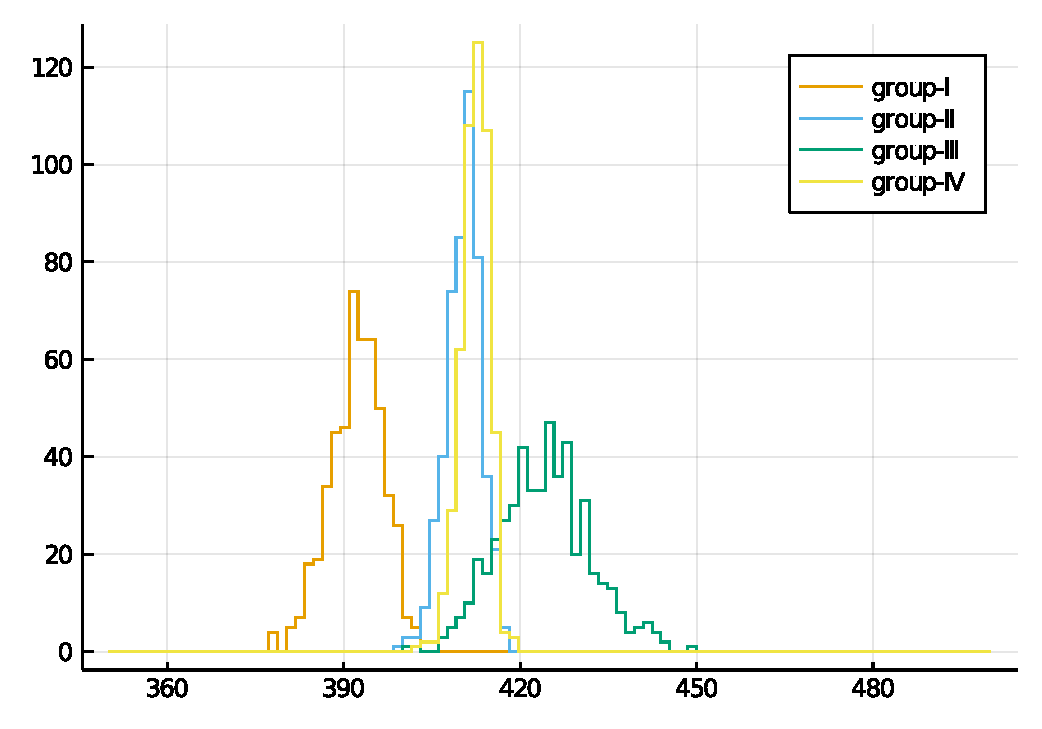
\includegraphics[width=0.48\textwidth]{llh_testing_higgs.pdf}
  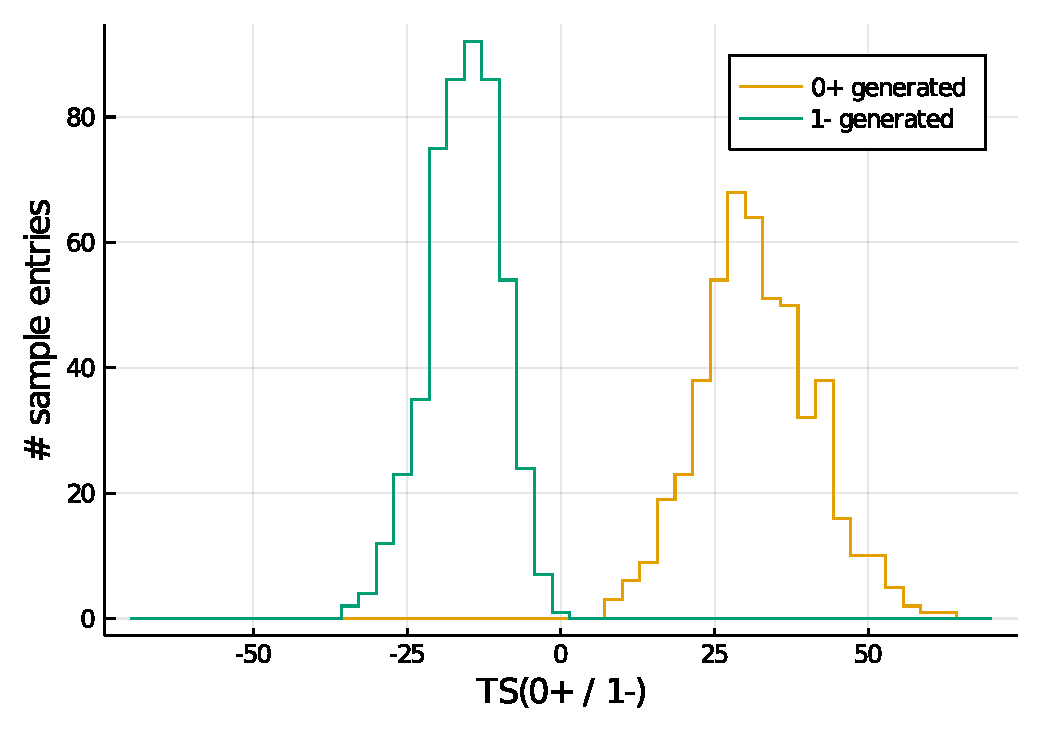
\includegraphics[width=0.48\textwidth]{TS_0p_vs_1m.pdf}
  \caption{The left plot shows the distribution the
  log-likelihood functions maximized on the simulated samples of the $H\to Z^0(\mu^+\mu^-)Z^0(\mu^+\mu^-)$ decay (the $J^P=0^+$ pool, see the text).
  The distribution of the test statistics $\TS(0^+|1^-)$ for the $J^P=0^+$ pool and the $J^P=1^-$ pool are drawn on the right plot by orange and green lines, respectively.}
  \label{fig:TS.fixedH}
\end{figure}
One sees that the group-$\I$ hypothesis has the highest likelihood in average.
The separation is even larger once the test statistics from Eq.~\eqref{eq:test.statistics} is computed for each sample.
The orange distribution on the right panel of Fig.~\ref{fig:TS.fixedH} shows the comparison of the group-$\I$ hypothesis with the selected alterative hypotheses that is taken to be the group-$\III$.
% The distribution of $\TS_{0^+/1^-}$ over the pool is entirely above zero.
Test statistics on the $1^-$ generated data, i.e. the green distribution on the right panel of Fig.~\ref{fig:TS.fixedH}, is calculated by creating the second pool corresponding to the matrix $H_\III$ with $a = 1/2$.
As expected, the $1^-$ hypothesis is found to have the highest likelihood in average over the second pool. The green distribution in right panel of Fig.~\ref{fig:TS.fixedH} is largely negative.

As stressed above, an important part of the separation power comes from the $\Delta\phi$ distribution.
Fig.~\ref{fig:higgs.phi} an example of $I(\Delta\phi)$ for the two combined sample of the first pool.
\begin{figure}
  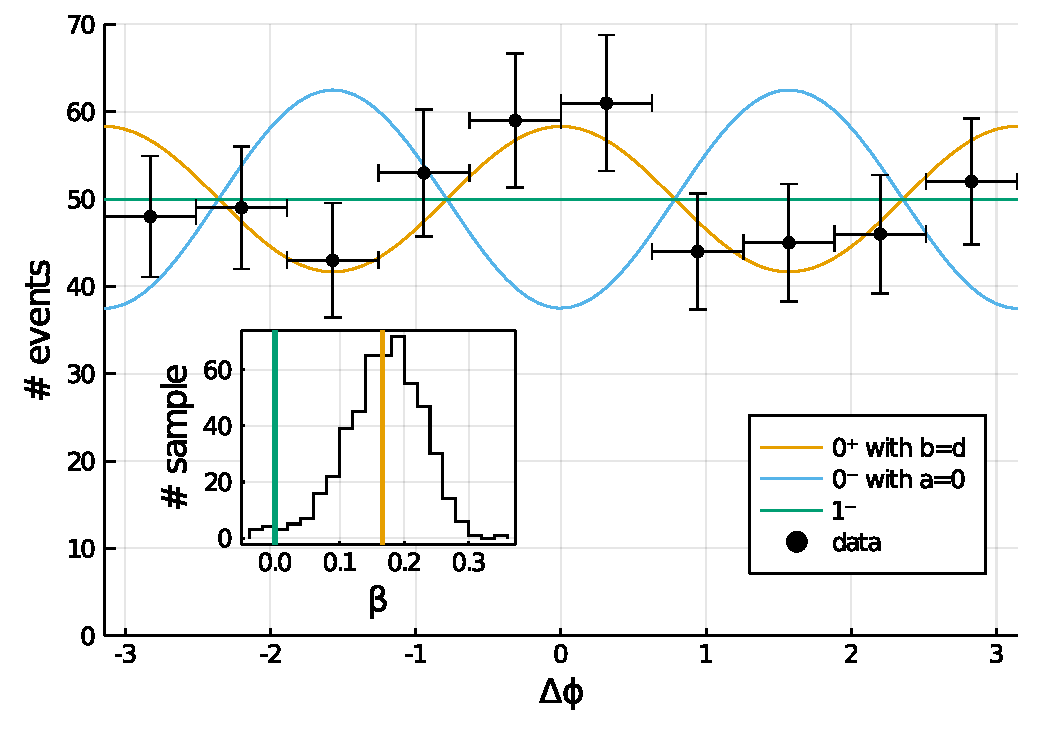
\includegraphics[width=0.48\textwidth]{phi_higgs.pdf}
  \caption{The distribution of the polar angle $\Delta\phi$ for the Higgs decay to $\mu^+\mu^-\mu^+\mu^-$ with $1000$ simulated events is labeled by "data".
  The orange line is the expectation curve under the $J^P=0^+$ hypotheses with $b=d=1/\sqrt{3}$.
  The distribution is flat when $J$ is odd.
  The blue line gives an example of the even-unnatural $J^P$ quantum numbers (group-\II).}
  \label{fig:higgs.phi}
\end{figure}

\section{Conclusion}
We have derived an amplitude for the hadronic production of two identical vector-meson system in a model-independent framework.
For well-definite $J^P$ quantum numbers, angular distributions is inhomogeneous
and differ depending on the parity of $J$ and the naturality of $J^P$.
We showed that four groups of $J^P$ can be distinguish based on angular distributions.
The test-statistics discriminator is proposed.
The power of the three-dimensional analysis is demonstrated using the Standard Model Higgs decay to a pair of the $Z$ bosons.

\section*{Acknowledgement}
The project was motivated by a discussion in the LHCb Amplitude Analysis group.
We thank Biplab Day for organizing seminar dedicated to $X\to VV$.
We would like to gratefully thank Alessandro Pilloni for useful comments on the work.
We thank Liupan An and Ronan McNulty for useful discussions and help with the paper draft.

\appendix

\section{Modifications for $X\to V(S^+S^-)V(S^+S^-)$} \label{sec:KKKK}

The amplitude requires a small modification when a system of four scalar particles is considered,
e.g. $\phi\phi$ decaying to four kaons.
The decay matrix element in Eq.~\eqref{eq:decay.A} reads:
\begin{align}
  A^{\nu}_{4S}(\theta_1,\theta_2,\Delta\phi) &= 3
  \sum_{\lambda_1,\lambda_2}
  \delta_{\nu,\lambda_1-\lambda_2} (-1)^{1-\lambda_2}
  H_{\lambda_1\lambda_2}
  d_{\lambda_1,0}^{1}(\theta_1) d_{\lambda_2,0}^{1}(\theta_2)
  e^{i\lambda_2 \Delta\phi}
\end{align}
where the decay $V\to S^+S^-$ proceeds in $P$-wave only.
As there is no averaging over the final-particles spin,
the variation in the $\Delta\phi$-dependence is more pronounced.
\begin{align}
  I_{4S}(\Delta\phi) = 1
   + 2 h_{1,1} h_{-1,-1}^* \cos(2 \Delta\phi).
\end{align}
% with $N_{4S}$ being the total number of the observed events.
\mishatodo{Add $\cos\theta_1$ distribution for $4K$.}

\section{Polarization vectors} \label{sec:polarisation.vectors}

To translate a covariant expression in Eq.~\eqref{eq:HZZ} to helicity amplitude
the explicit expressions for the polarization vectors are used:
\begin{align}
  \varepsilon_z^{\mu}(\pm1) &= \frac{1}{\sqrt{2}} \left( 0,\mp 1,-i,0 \right), &
  \varepsilon_z^{\mu}(0) &= \frac{1}{m_Z} \left(p,0,0,E\right),
\end{align}
where $E$, $p$, and $m_Z$ are the energy, momentum, and mass of the $Z$ boson, respectively.
The general expressions for the rotational vectors follow:
\begin{align}
  % \varepsilon_1(\pm1) &= R_z(\Delta\phi) R_y(\theta) (0,-i,\mp 1,0)\frac{1}{\sqrt{2}},\\
  % \varepsilon_2(\pm1) &= R_z(\Delta\phi) R_y(\theta) R_y(\pi) (0,-i,\mp 1,0)\frac{1}{\sqrt{2}};\\
  % \varepsilon_1(0) &= R_z(\Delta\phi) R_y(\theta) (-p,0,0,E)\frac{1}{m},\\
  % \varepsilon_2(0) &= (-1) R_z(\Delta\phi) R_y(\theta) R_y(\pi) (-p,0,0,E)\frac{1}{m},
  \varepsilon_1(\lambda) &= R_z(\phi) R_y(\theta) \varepsilon_z(\lambda),\\
  \varepsilon_2(\lambda) &= (-1)^{1-\lambda} R_z(\phi) R_y(\theta) R_y(\pi) \varepsilon_z(\lambda),\\
\end{align}
where $R_y(\phi)R_y(\theta)$ is a product of the three-dimensional rotation matrices
that transforms the vector $(0,0,1)$ to the direction $(\sin\theta\cos\phi,\,\sin\theta\sin\phi,\,\cos\theta)$.
The second particle requires additional rotation by $\pi$ about the $y$ axis.
We also use the particle-2 phase convention that flips the sign of $\varepsilon_2(0)$.

\section{The $P s$ invariance} \label{sec:Ps.invariance}
The helicity coupling matrices from different groups in Eq.~\eqref{eq:matrices} do not overlap;
moreover, they are all orthogonal to each other.
Nevertheless, there are potential cases where different hypothesis are not distinguishable.
An example that demonstrate such degeneracy is the following:
\begin{equation}
  H^{(\text{deg.})} = \begin{pmatrix}
    0 &1 &0 \\
    s & 0 &sP \\
    0 &P &0
  \end{pmatrix},
\end{equation}
where $s$ is the parity of $J$, and $P$ is the naturality of $J^P$.
The matrix of this type is present in all groups for different values of $s$ and $P$
The intensity of the unpolarized decay can be computed explicitly~\cite{SymPy}:
\begin{align}
  I(H) &= \frac{s^{2} P^{2} \sin^{2}{\left (\theta_{1} \right )} \cos^{2}{\left (\theta_{2} \right )}}{2} + \frac{s^{2} P^{2} \sin^{2}{\left (\theta_{1} \right )}}{2} + \frac{s^{2} \sin^{2}{\left (\theta_{1} \right )} \cos^{2}{\left (\theta_{2} \right )}}{2} + \frac{s^{2} \sin^{2}{\left (\theta_{1} \right )}}{2} \\ \nonumber
   &\quad + \frac{s P \left(\cos{\left (- 2 \theta_{1} + 2 \theta_{2} + \Delta\phi \right )} + \cos{\left (2 \theta_{1} - 2 \theta_{2} + \Delta\phi \right )} - \cos{\left (2 \theta_{1} + 2 \theta_{2} - \Delta\phi \right )} - \cos{\left (2 \theta_{1} + 2 \theta_{2} + \Delta\phi \right )}\right)}{8}\\ \nonumber
   &\quad+\frac{P^{2} \sin^{2}{\left (\theta_{2} \right )} \cos^{2}{\left (\theta_{1} \right )}}{2} + \frac{P^{2} \sin^{2}{\left (\theta_{2} \right )}}{2} + \frac{\sin^{2}{\left (\theta_{2} \right )} \cos^{2}{\left (\theta_{1} \right )}}{2} + \frac{\sin^{2}{\left (\theta_{2} \right )}}{2}
\end{align}
The expression does not change under the flip of $P$ and $s$ sign simultaneously.
Hence, group-$\II$ with $b=0$ is undistinguished from group-$\III$,
and group-$\I$ with $b=d=c=0$ have the same angular distributions as group-$\IV$ with $c=0$.
Such vanishing of the helicity couplings, however, must be an exceptional case indicating some peculiar physical reason.

\bibliography{ref}
\end{document}




% \begin{align}
%   \frac{\diff^2 N}{\diff \cos\theta_1\,\diff \cos\theta_2} =
%   |H_{\lambda_1\lambda_2}|^2
%   \sum_{\xi_1,\xi_2}^{\{-1,1\}}
%   9|d_{\lambda_1,\xi_1}^{1}(\theta_1) d_{\lambda_2,\xi_2}^{1}(\theta_2)|^2.
% \end{align}

% \section{LS couplings}
%
% \begin{align}
%   H_{\lambda_1,\lambda_2} = (-1)^{j_2-\lambda_2} \sum_{ls} \sqrt{\frac{2l+1}{2j+1}}
%   \left\langle 1,\lambda_1;1,\lambda_2|s,\lambda_1-\lambda_2 \right\rangle
%   \left\langle L,0;s,\lambda_1-\lambda_2|j,\lambda_1-\lambda_2 \right\rangle H_{ls}.
% \end{align}
%
% \begin{align*}
%   1^-\otimes 1^-: && S:\qquad & {\color{cola} 0^+}\quad {\color{colb} 1^+}\quad {\color{colc} 2^+},\\
%                   && P:\qquad & \color{gray} 1^-\quad (0^-,1^-,2^-)\quad (1^-,2^-,3^-),\\
%                   && D:\qquad & {\color{colc} 2^+}\quad ({\color{colb} 1^+},{\color{colc} 2^+},3^+)\quad ({\color{cola} 0^+},{\color{colb} 1^+},{\color{colc} 2^+},3^+,4^+),\\
%                   && F:\qquad & \color{gray} 3^-\quad (2^-,3^-,4^-)\quad (0^-,1^-,2^-,3^-,4^-),\\
%                   && H:\qquad & 4^+\quad (3^+,4^+,5^+)\quad ({\color{colc} 2^+},3^+,4^+,5^+,6^+).
% \end{align*}

% \section{Odd and even spins}

% \begin{figure}
%   \includegraphics[width=0.46\textwidth]{../plots/moment_M2phi_Nev=500.pdf}
%   \caption{Distribution of $M_{\cos(2\Delta\phi)}$ for a sample of random coupling constants.
%   A sample of $500$ events is generated for every hypothesis of couplings.}
%   \label{}
% \end{figure}
%
% \begin{figure}
%   \includegraphics[width=0.9\textwidth]{../plots/llh_of_fit_of_J012.pdf}
%   \caption{Hypothesis testing with $500$ events}
%   \label{fig.3dfit}
% \end{figure}


% Matrices of couplings without the phase $(-1)^{j_2-\lambda_2}$ are symmetric (round brackets) or asymmetric (square parentheses)
% \begin{itemize}
%   \item $j = 0$:
% \begin{align*}
%   % l = 0, s = 0
%   \frac{\sqrt{3}}{3}
%   \begin{pmatrix}1 & 0 & 0\\0 & -1 & 0\\0 & 0 & 1\end{pmatrix}&&
%   % l = 2, s = 2
%   \frac{\sqrt{6}}{6}
%   \begin{pmatrix}1 & 0 & 0\\0 & 2 & 0\\0 & 0 & 1\end{pmatrix}
% \end{align*}
%   \item $j = 1$:
% \begin{align*}
%   % l = 0, s = 1
%   \frac{\sqrt{6}}{6}
%   \begin{pmatrix}-1 & -1 & 0\\-1 & 0 & 1\\0 & 1 & 1\end{pmatrix}&&
%   % l = 2, s = 1
%   \frac{\sqrt{3}}{6}
%   \begin{pmatrix}2 & -1 & 0\\-1 & 0 & 1\\0 & 1 & -2\end{pmatrix}&&
%   % l = 2, s = 2
%   \frac{1}{2}
%   \left[\begin{matrix}0 & -1 & 0\\1 & 0 & -1\\0 & 1 & 0\end{matrix}\right]
% \end{align*}
% \item $j = 2$:
% \begin{align*}
%   % l = 0, s = 2
%   \frac{\sqrt{30}}{30}
%   \begin{pmatrix}1 & \sqrt{3} & \sqrt{6}\\\sqrt{3} & 2 & \sqrt{3}\\\sqrt{6} & \sqrt{3} & 1\end{pmatrix}&&
%   % l = 2, s = 0
%   \frac{\sqrt{3}}{3}
%   \begin{pmatrix}1 & 0 & 0\\0 & -1 & 0\\0 & 0 & 1\end{pmatrix}&&
%   % l = 2, s = 1
%   \frac{1}{2}
%   \left[\begin{matrix}0 & -1 & 0\\1 & 0 & 1\\0 & -1 & 0\end{matrix}\right]&&
%   % l = 2, s = 2
%   \frac{\sqrt{7}}{14}
%   \begin{pmatrix}- \frac{2 \sqrt{3}}{3} & -1 & 2 \sqrt{2}\\-1 & -\frac{4 \sqrt{3}}{3} & -1\\2 \sqrt{2} & -1 & - \frac{2 \sqrt{3}}{3}\end{pmatrix}&&
%   % l = 4, s = 2
%   \frac{\sqrt{70}}{70}
%   \begin{pmatrix}\sqrt{6} & -2 \sqrt{2} & 1\\- 2 \sqrt{2} & 2\sqrt{6} & - 2 \sqrt{2}\\1 & -2\sqrt{2} & \sqrt{6}\end{pmatrix}
% \end{align*}
% \end{itemize}
%
% \begin{figure}
%   \includegraphics[width=0.195\textwidth]{../plots/map_JLS_000.pdf}
%   \includegraphics[width=0.195\textwidth]{../plots/map_JLS_022.pdf}
%   \caption{}
%   \label{fig.j0}
% \end{figure}
% \begin{figure}
%   \includegraphics[width=0.195\textwidth]{../plots/map_JLS_101.pdf}
%   \includegraphics[width=0.195\textwidth]{../plots/map_JLS_121.pdf}
%   \includegraphics[width=0.195\textwidth]{../plots/map_JLS_122.pdf}
%   \caption{}
%   \label{fig.j1}
% \end{figure}
% \begin{figure}
%   \includegraphics[width=0.195\textwidth]{../plots/map_JLS_202.pdf}
%   \includegraphics[width=0.195\textwidth]{../plots/map_JLS_220.pdf}
%   \includegraphics[width=0.195\textwidth]{../plots/map_JLS_221.pdf}
%   \includegraphics[width=0.195\textwidth]{../plots/map_JLS_222.pdf}
%   \includegraphics[width=0.195\textwidth]{../plots/map_JLS_242.pdf}
%   \caption{}
%   \label{fig.j2}
% \end{figure}


% \begin{align}
%     I(\cos\theta_1,\phi_1,\cos\theta_2,\phi_2) &= 9\sum_{M}P_M
%     \sum_{\lambda_1,\lambda_2}\sum_{\lambda_1',\lambda_2'}
%     d_{M,\lambda_1-\lambda_2}^{J}(\theta) (-1)^{1-\lambda_2}
%     d_{M,\lambda_1'-\lambda_2'}^{J}(\theta) (-1)^{1-\lambda_2'}
%     \\ \nonumber
%     &\qquad\times
%     H_{\lambda_1\lambda_2} H_{\lambda_1'\lambda_2'}^{*}
%     e^{i(\lambda_1'-\lambda_1)\phi_1}
%     e^{i(\lambda_2'-\lambda_2)\phi_2}
%     \\ \nonumber
%     &\qquad\times
%     \sum_{\xi_1}^{\{-1,1\}}
%     d_{\lambda_1,\xi_1}^{1}(\theta_1) d_{\lambda_1',\xi_1}^{1}(\theta_1)
%     \sum_{\xi_2}^{\{-1,1\}}
%     d_{\lambda_2,\xi_2}^{1}(\theta_2) d_{\lambda_2',\xi_2}^{1}(\theta_2).
% \end{align}
